\chapter{Methodology}
\section{Time to Digital Converter}

\subsection{specifications}
The main specifications for the TDC are the following:
\begin{itemize}
    \item Corner set up: TT, 60$^{\circ}$C, 1.2 V
    \item Clock reference frequency: 100 MHz
    \item Number of bits: 4
    \item Acquisition range: -2$\pi$ to 2$\pi$
\end{itemize}

The TDC implements a 4-bit flash architecture for a time resolution of 625 ps ($\Delta$) in each half of the clock period. The acquisition range is 20 ns, which corresponds to a phase 
range of -2$\pi$ to 2$\pi$ for a clock frequency of 100 MHz.

\subsection{Architecture}
The TDC architecture is based on the design presented in \cite{bib:tdc_flash}. The core of the TDC consist of a voltage-controlled delay line (VCDL), a set of D flip-flops to sample the
state of the VCDL, and a thermometer-to-binary decoder that process the sampled data to produce a workable digital output. This arrangement is used twice, once for the case when the
feedback signal has a lower frequency (or delayed phase) than the reference clock, and the other for the case when the feedback signal has a higher frequency (or advanced phase) than
the reference clock. The two outputs are then combined to produce the final output of the TDC. Such an architecture (Fig. \ref{fig:TDC_conventional_architecture}) would be the 
conventional way to implement a TDC that reads both cases for the phase difference between the reference clock and the feedback signal. 

\begin{figure}[h]
    \centering
    \includegraphics[width=1\textwidth]{figures/TDC_conventional_architecture.png}
    \caption{Conventional TDC architecture}
    \label{fig:TDC_conventional_architecture}
\end{figure}

The architecture of figure \ref{fig:TDC_conventional_architecture} has shortcomings, such as the fact that it does not allow for a phase difference of more than 2$\pi$ between the
reference clock and the feedback signal, meaning that the TDC will not be able to read the phase difference beyond half cycle for each clock period. This is limiting for the PLL, as it
would not be able to correct the phase difference if it exceeds $\pi$ for each case. To overcome this limitation and achieve the desired acquisition range set in the specifications, 
the TDC architecture of figure \ref{fig:TDC_proposed_architecture} is proposed.

\begin{figure}[h]
    \centering
    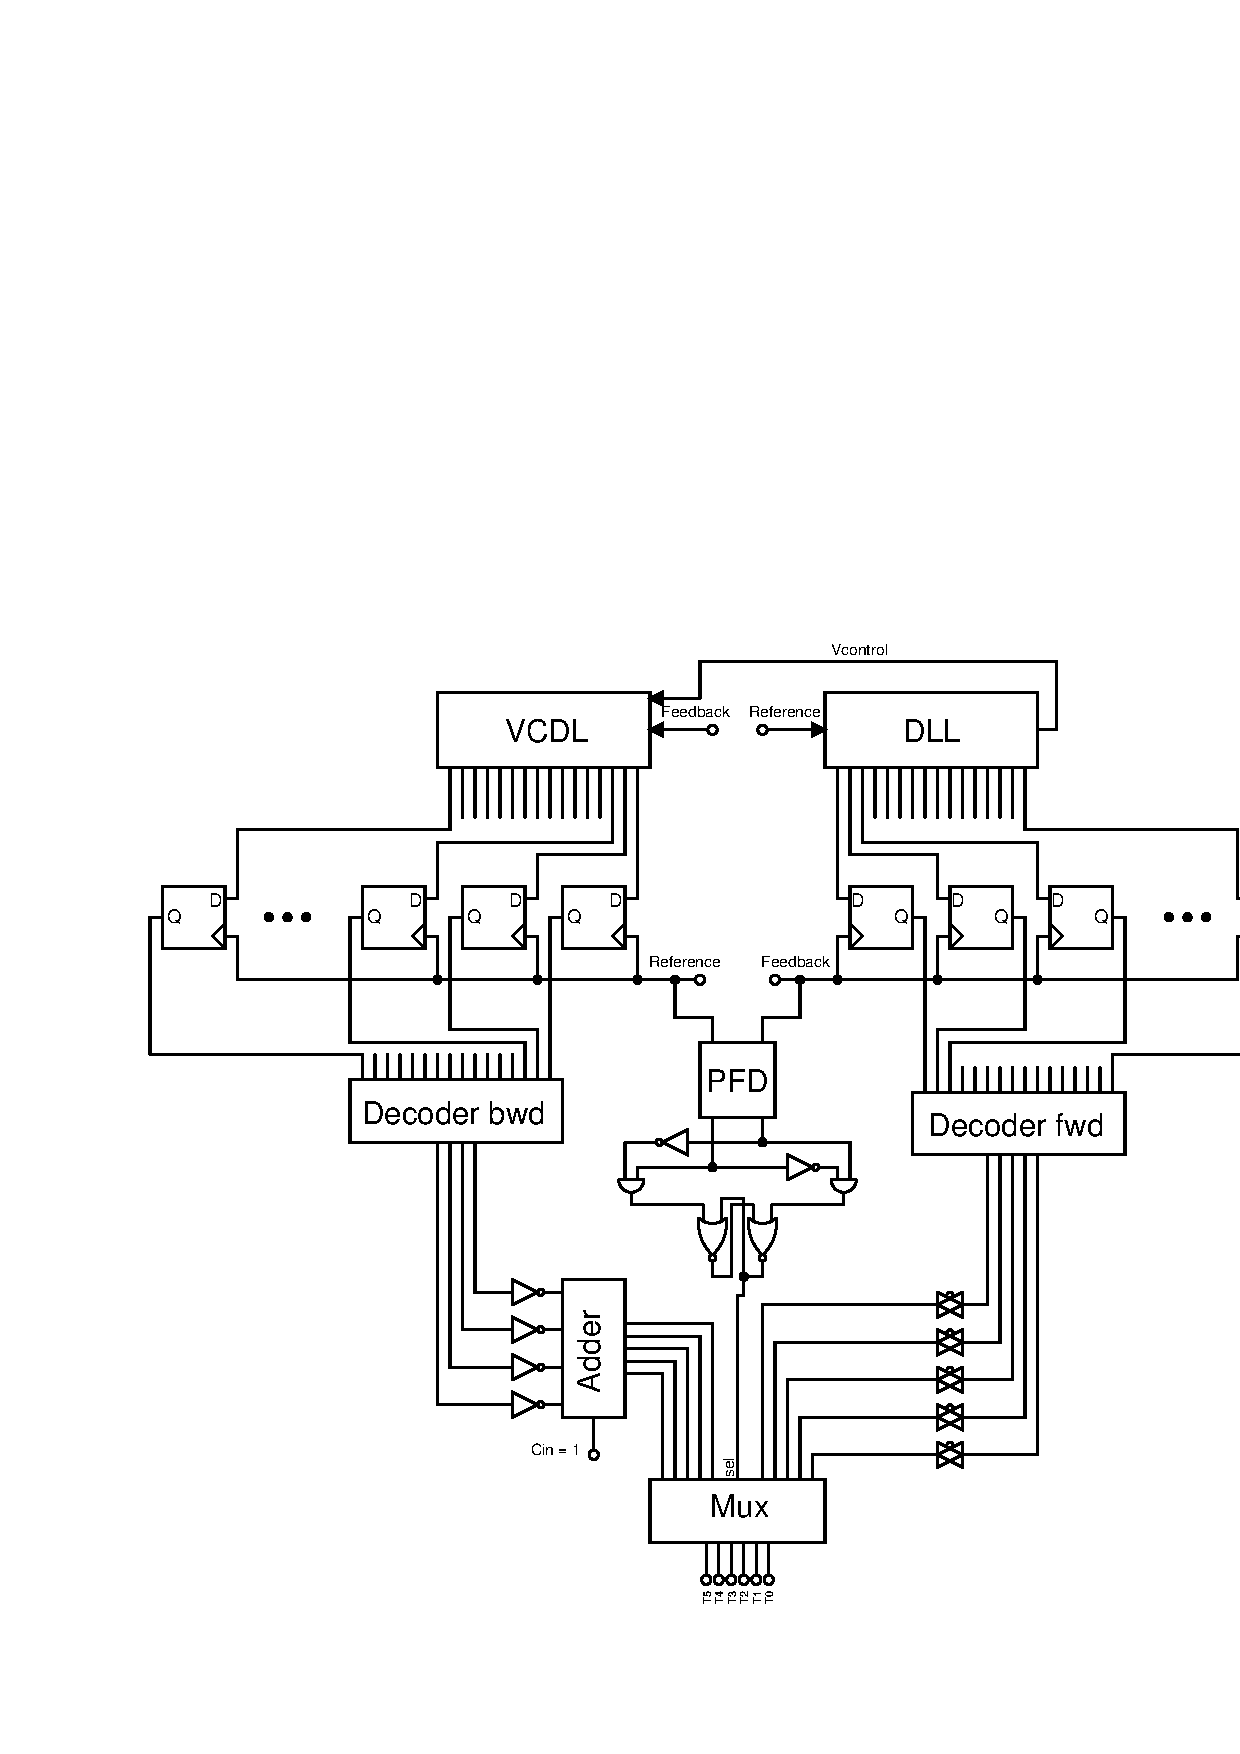
\includegraphics[width=1\textwidth]{figures/TDC_proposed_architecture.png}
    \caption{Proposed TDC architecture}
    \label{fig:TDC_proposed_architecture}
\end{figure}

The main differences between the conventional architecture and the proposed one are that the latter uses a DLL instead of a VCDL to implement the delay line, a slight modification
to the thermometer-to-binary decoder, and a different way to combine the outputs of the two TDCs.

The DLL allows for a more robust and stable delay line as it is less sensitive to PVT variations. This is important for the PLL, as it needs to be able to operate under different
conditions and still be able to correct the phase difference between the reference clock and the feedback signal.

The thermometer-to-binary decoder is modified to allow for the reading of both cases of the phase/frequency difference between the signals. This is the main way that the TDC is able
to read a phase difference of more than 2$\pi$ each cycle and as far as the author is aware, this is the first time that such a modification has been proposed in the literature.

Finally, the outputs of the two TDCs are combined using a multiplexer that selects the output based on the frequency state of the feedback signal. The selector needs to be able to
determine whether the feedback signal is leading or lagging the reference clock, which is done by retrieving the information lost because of the decoder modification.


All of this changes done to the conventional TDC architecture will be further explained in the following sections of this chapter, where the design of the TDC will be presented in 
detail.

\subsection{System behavior}
Both architectures have the same principle of operation and each of their blocks have the same behavior. Both architectures have some sort of delay line that measures the phase difference
between the reference clock and the feedback signal, a thermometer-to-binary decoder that processes the sampled data to produce a workable digital output, and both have the same number of 
D flip-flops to sample the state of the delay line which is equal to $2^n-1$ where $n$ is the number of bits of the TDC.

The operation of the TDC of \ref{fig:TDC_conventional_architecture} is as follows: When the rising edge of the reference clock occurs and a new cycle starts, the circuit in charge of reading the 
case where the feedback signal is lagging (forward) with respect to the reference will start its operation, meaning that its VCDL will be reset and start counting the delay until the next rising 
edge of either the reference clock or the feedback signal occurs. If the former occurs first, then the circuit in charge of reading the case where the feedback signal is leading (backward) will 
never start its operation and the TDC output will be the same as the last cycle. If the latter occurs first, then the backward circuit will start its operation and count the remaining delay until
the next rising edge of the reference clock and the TDC output will be the subtraction of the forward output minus the backward output.

Because the decoders of the TDC of figure \ref{fig:TDC_conventional_architecture} are thermometer-to-binary decoders, their output is equal to 0 after half of the reference clock period time has
passed, meaning the result of the TDC will be either the forward output or the 2's complement of the backward output depending on which of the half cycle of the clock period the feedback signal
occurs. This feature is what allows the TDC to detect whether the feedback signal is leading or lagging the reference clock, but it is also what limits the TDC to a phase difference of $\pm \pi$
each cycle.

\begin{figure}[H]
    \centering
    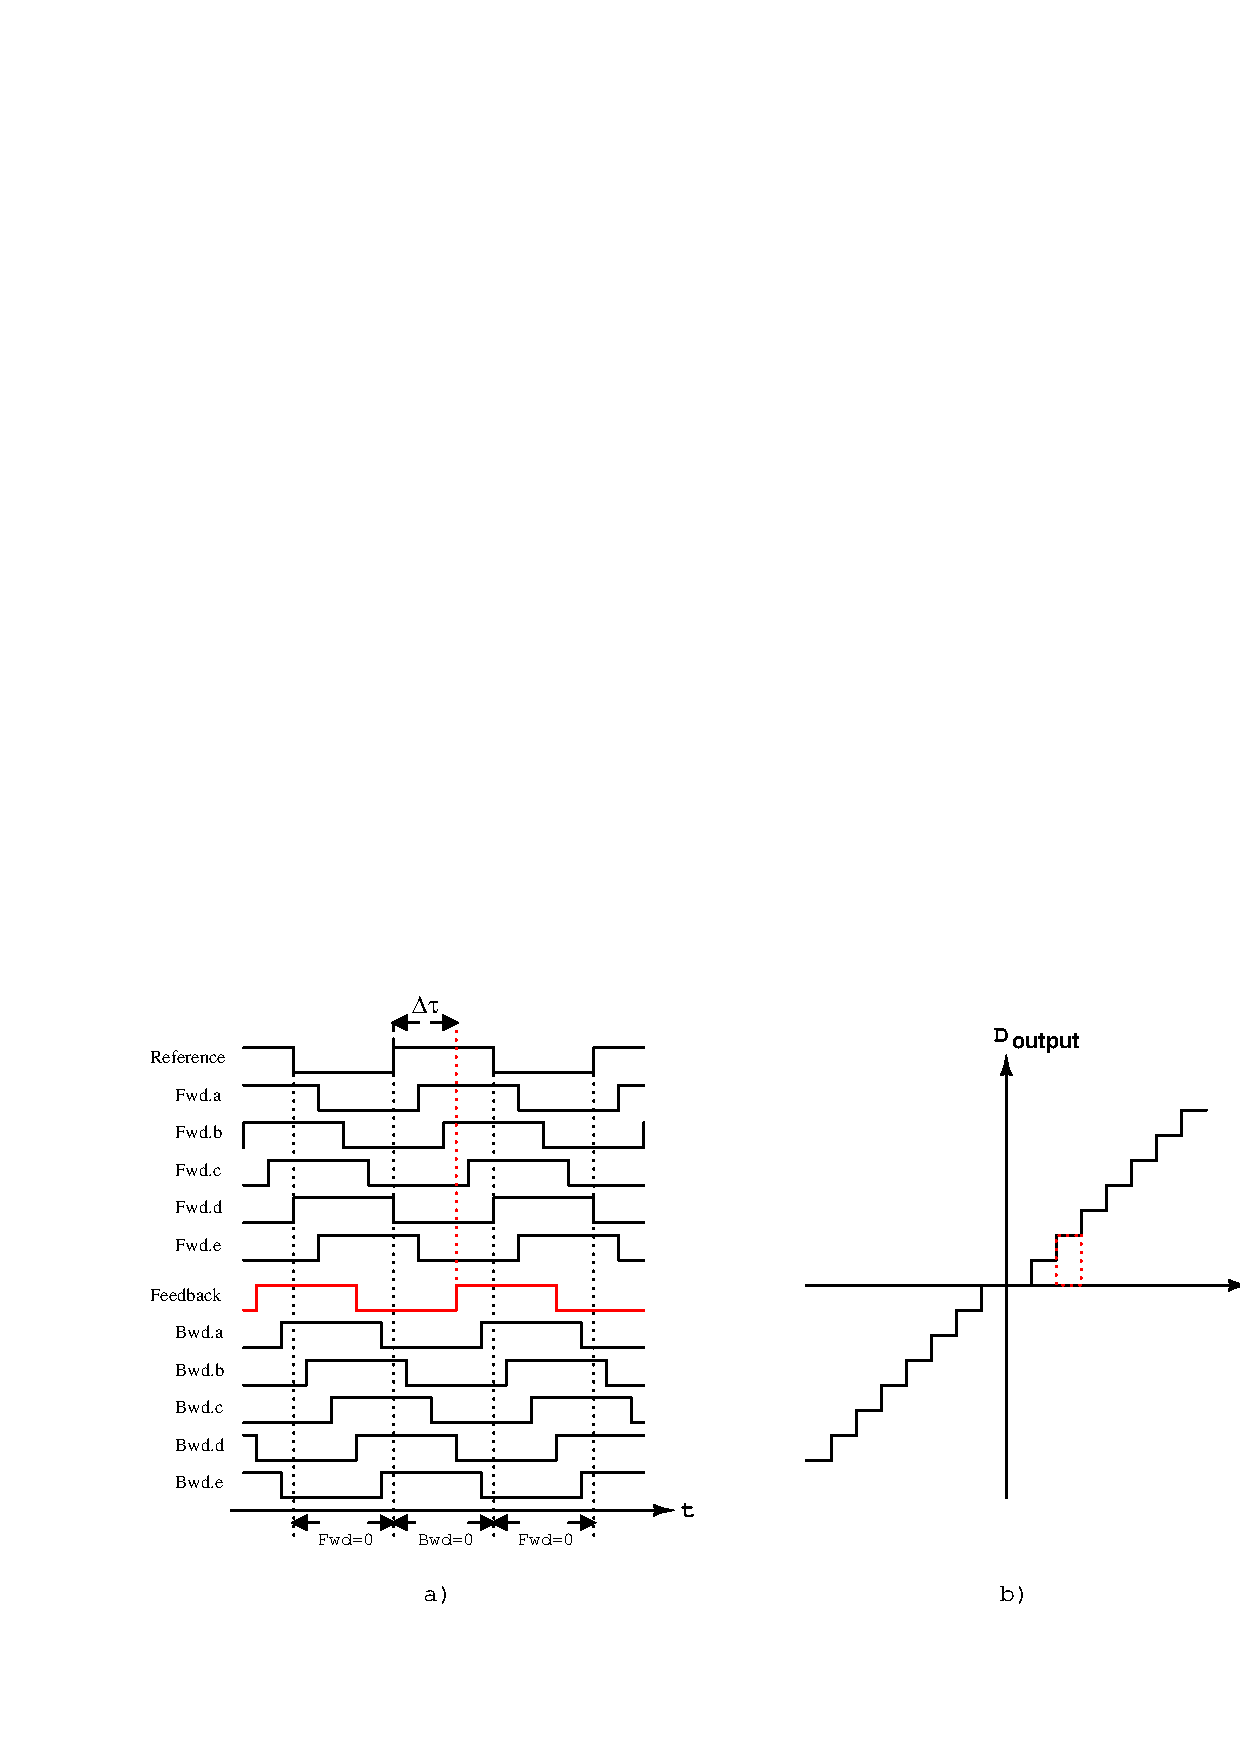
\includegraphics[width=1\textwidth]{figures/TDC_timing_diagram.png}
    \caption{a) Conventional TDC timing diagram for a positive phase error, and b) its ideal characteristic.}
    \label{fig:TDC_conventional_timing_diagram}
\end{figure}

Figure \ref{fig:TDC_conventional_timing_diagram} further elaborates on this point, showing the timing diagram and the ideal characteristic of the conventional architecture. Notice that there 
is a 0 gain zone around zero delay where the TDC will not be able to detect small phase differences, also notice that the output will only take values between 7 and -7 for a 4-bit TDC. Both of
these issues are addressed in the proposed architecture.

\subsection{Design}
The design for the TDC proposed in this work is approached in a modular way, where each block is designed separately and then integrated into the final TDC. Even though differences exist between
both paths (forward and backward) of the TDC, the blocks are the exact same for both, meaning that the design can be done in a single step and then replicated for each path with
slight modifications.

\subsubsection{DLL}
The implementation of the DLL is that of figure \ref{fig:DLL_architecture}, which is based on \cite{bib:DLL_Razavi_paper}. The DLL is composed of a voltage-controlled delay line (VCDL) that is used
to measure the phase difference between the reference clock and the feedback signal, a charge pump that is used to control the delay of the VCDL, and a phase frequency detector (PFD) that is used to
determine whether the feedback signal is leading or lagging the reference clock.

\paragraph{VCDL}
The delay elements of the VCDL are implemented using a series of CMOS inverters whose delay is controlled by two variable resistors at the source of each transistor (see Fig. \ref{fig:VCDL_delay_elements}).
Each one of this elements must have a delay equal to 625 ps for a total of 10 ns (the period of the reference clock) after 16 of them. 625 ps is a relatively high amount of delay for a CMOS inverter of
minimum dimensions in 65 nm, there are multiple approaches towards meeting such a high delay, but the preferable method from the perspective of optimizing the phase noise according to \cite{bib:Razavi_PLL_book}
is to increase the number of stages.

Therefore after simulating the circuit of figure \ref{fig:VCDL_delay_elements} and measuring its delay (for a load of another identical inverter) it was determined that the number of stages necessary to achieve
625 ps in each delay element is 38. The dimensions for all 6 MOSFETs are annotated in table \ref{tab:VCDL_delay_elements_dimensions}.


\paragraph{Charge pump}
\paragraph{PFD}

\subsubsection{D flip-flops}

\subsubsection{modified thermometer-to-binary decoders}

\subsubsection{PFD selector circuit}

\subsubsection{multiplexer}

\section{Digitally controlled oscillator}

\section{Digital loop filter}
